\chapter{Les éléments dans l'Univers et sur la Terre}\label{ch:g9:elements-universe-earth}

Le calcium de tes os, le fer de ton sang et l'oxygène que tu respires
n'ont pas été fabriqués sur la Terre. Ils l'ont été au cœur d'étoiles qui
ont vécu et sont mortes avant la naissance du Soleil, et ils passent
depuis des milliards d'années de la roche à la mer, de la mer à la
plante, de la plante à l'animal. Certains éléments sont partout,
d'autres sont rares. Quels éléments composent les étoiles, la Terre, les
océans --- et nous-mêmes~?

\begin{recall}
Un \omterm{def:g9:inside-the-atom:element}{élément chimique} est l'ensemble des \omterm{def:g7:atoms-and-molecules:atom}{atomes} qui ont le même \omterm{def:g9:inside-the-atom:atomic-number}{numéro
atomique} $Z$~; la masse d'un \omterm{def:g7:atoms-and-molecules:atom}{atome} est proche de
$A \times \qty{1.67e-27}{kg}$, où $A$ est son \omterm{def:g9:inside-the-atom:atomic-number}{nombre de masse}
(\cref{ch:g9:inside-the-atom}). Le \omterm{def:g9:periodic-table-first-look:periodic-table}{tableau périodique} range les
118 éléments par \omterm{def:g9:inside-the-atom:atomic-number}{numéro atomique}
(\cref{ch:g9:periodic-table-first-look}). L'\omterm{def:g4:air-a-mixture-of-gases:air}{air} contient environ quatre
cinquièmes de diazote et un cinquième de dioxygène
(\cref{ch:g4:air-a-mixture-of-gases}).
\end{recall}

\section{Les éléments des étoiles}

\begin{definition}[Abondance]\label{def:g9:elements-universe-earth:abundance}
L'\emph{abondance}\index{abondance} d'un élément dans un corps --- une
étoile, la croûte terrestre, l'océan, un être vivant --- est sa part de
la masse totale, en général donnée en pourcentage.
\end{definition}

\begin{proposition}[Le Soleil, c'est de l'hydrogène et de l'hélium]\label{prop:g9:elements-universe-earth:sun}
% ledger: ab:sun-X, ab:sun-Y, ab:sun-Z
La surface du Soleil est constituée, en masse, d'environ
\qty{74}{\percent} d'hydrogène et de \qty{25}{\percent} d'hélium~; tous
les autres éléments réunis n'en représentent qu'environ
\qty{1.3}{\percent}. La plus grande partie de la matière visible de
l'Univers a une composition semblable~: de l'hydrogène et de l'hélium,
avec une pincée de tout le reste.
\end{proposition}

\begin{proposition}[Des éléments fabriqués dans les étoiles]\label{prop:g9:elements-universe-earth:stars}
L'hydrogène et la plus grande partie de l'hélium se sont formés dans les
premières minutes de l'Univers. Presque tous les éléments plus lourds
--- le carbone, l'oxygène, le fer, l'or --- ont été fabriqués plus tard,
au cœur des étoiles, puis dispersés dans l'espace quand ces étoiles ont
explosé. De nouvelles étoiles et de nouvelles planètes se sont formées à
partir de cette poussière enrichie. La façon dont les étoiles s'y
prennent est racontée dans le livre de physique.
\end{proposition}

\begin{omfigure}
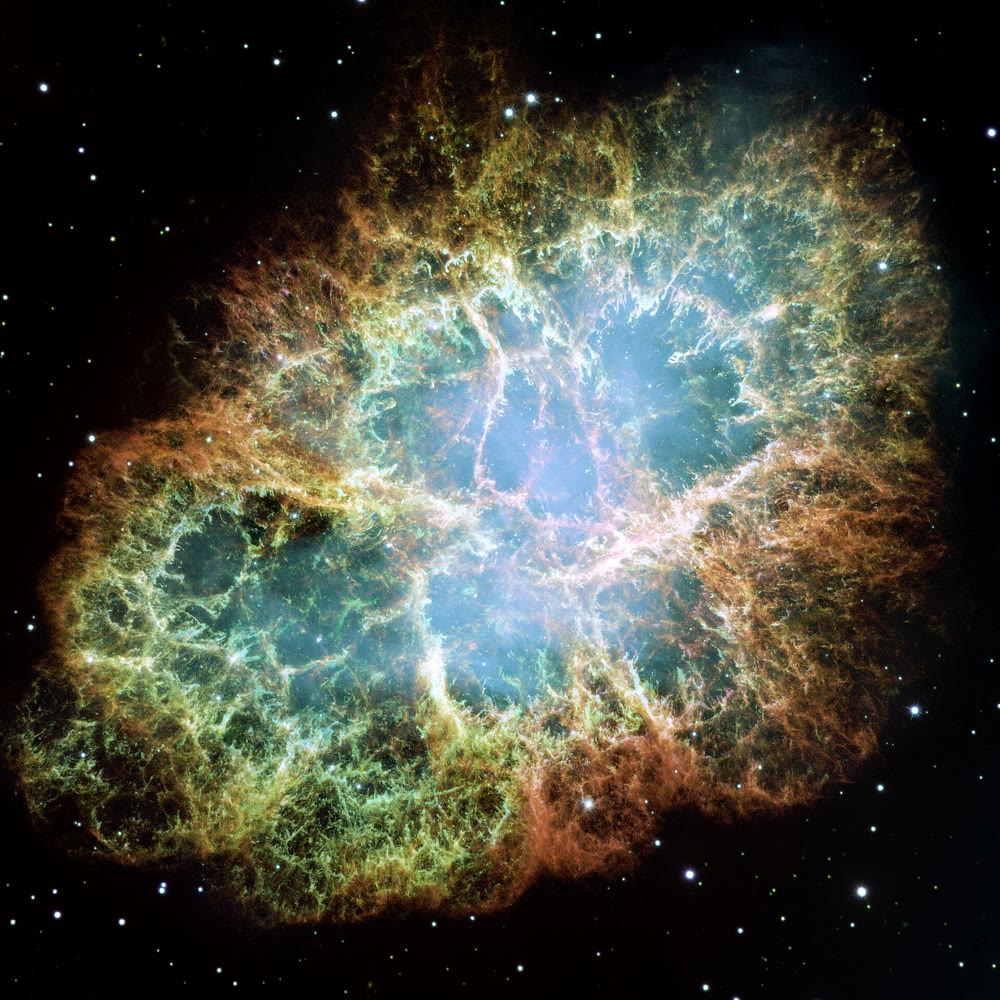
\includegraphics[width=0.45\linewidth]{images/book1/crab-nebula.jpg}

{\small La nébuleuse du Crabe, le nuage laissé par une étoile qui a
explosé il y a près de mille ans, et qui répand de nouveaux éléments
dans l'espace (NASA, ESA, J.~Hester et A.~Loll).}
\end{omfigure}

\section{La Terre}

\begin{proposition}[La croûte terrestre]\label{prop:g9:elements-universe-earth:crust}
% ledger: ab:crust-O, ab:crust-Si, ab:crust-Al, ab:crust-Fe, ab:crust-Ca, ab:crust-Na, ab:crust-K, ab:crust-Mg, ab:crust-first10
La fine peau rocheuse de la Terre, la croûte, est faite en masse de
presque la moitié d'oxygène et de plus d'un quart de silicium~: les
roches et le sable sont surtout des oxydes de silicium et de quelques
métaux. Huit éléments --- l'oxygène, le silicium, l'aluminium, le fer,
le calcium, le sodium, le potassium, le magnésium --- en représentent
environ \qty{99}{\percent}. L'hydrogène et l'hélium, si répandus dans les
étoiles, y sont rares~: ces gaz légers se sont échappés de la Terre
jeune.
\end{proposition}

\begin{remark}[L'intérieur de la Terre]\label{rem:g9:elements-universe-earth:core}
La croûte n'est pas toute la Terre. Le fer, lourd, s'est enfoncé vers le
centre quand la jeune Terre était en fusion~: le noyau terrestre est
surtout fait de fer, avec un peu de nickel.
\end{remark}

\begin{proposition}[Les océans et l'air]\label{prop:g9:elements-universe-earth:ocean}
% ledger: sea:salts-share, sea:NaCl-ions, sea:MgSO4-ions, air:N2, air:O2
L'eau de mer est surtout de l'eau --- de l'hydrogène et de l'oxygène ---,
avec environ \qty{3.5}{\percent} en masse de sels dissous. Parmi les
\omterm{def:g9:ions:ion}{ions} dissous, les \omterm{def:g9:ions:ion}{ions} chlorure et sodium représentent environ
\qty{85}{\percent}, les \omterm{def:g9:ions:ion}{ions} magnésium et sulfate encore
\qty{10}{\percent}. L'\omterm{def:g4:air-a-mixture-of-gases:air}{air} est surtout fait de diazote et de dioxygène.
\end{proposition}

\begin{omfigure}
\begin{tikzpicture}
\begin{axis}[xbar, width=0.40\linewidth, height=5.4cm, xmin=0, xmax=85,
    bar width=7pt, symbolic y coords={Mg,K,Na,Ca,Fe,Al,Si,O}, ytick=data,
    xlabel={pourcentage de la masse}, title={\small la croûte terrestre},
    nodes near coords, nodes near coords style={font=\scriptsize},
    tick label style={font=\small}, label style={font=\small},
    axis lines*=left, enlarge y limits=0.08]
% ledger: ab:crust-O, ab:crust-Si, ab:crust-Al, ab:crust-Fe, ab:crust-Ca, ab:crust-Na, ab:crust-K, ab:crust-Mg
\addplot[fill=omDef!45, draw=omDef] coordinates {(46.6,O) (27.7,Si) (8.1,Al)
  (5.0,Fe) (3.6,Ca) (2.8,Na) (2.6,K) (2.1,Mg)};
\end{axis}
\end{tikzpicture}\hfill
\begin{tikzpicture}
\begin{axis}[xbar, width=0.40\linewidth, height=5.4cm, xmin=0, xmax=85,
    bar width=7pt, symbolic y coords={{P},{N},{Ca},{H},{C},{O}}, ytick=data,
    xlabel={pourcentage de la masse}, title={\small un corps humain},
    nodes near coords, nodes near coords style={font=\scriptsize},
    tick label style={font=\small}, label style={font=\small},
    axis lines*=left, enlarge y limits=0.1]
% ledger: body:atoms-O, body:atoms-C, body:atoms-H, body:atoms-N, body:atoms-Ca, body:atoms-P (masses = atoms x atomic mass, over 70 kg)
\addplot[fill=omProp!45, draw=omProp] coordinates {(61.1,O) (22.9,C) (10.1,H)
  (1.3,N) (1.5,Ca) (0.7,P)};
\end{axis}
\end{tikzpicture}

{\small \omterm{def:g9:elements-universe-earth:abundance}{Abondances} en masse. À gauche~: les huit principaux éléments de
la croûte terrestre. À droite~: les six principaux éléments du corps
d'un adulte mince (calculés à partir d'estimations du nombre d'\omterm{def:g7:atoms-and-molecules:atom}{atomes}).}
\end{omfigure}

\section{Le corps humain}

\begin{proposition}[Ce dont nous sommes faits]\label{prop:g9:elements-universe-earth:body}
% ledger: body:atoms-O, body:atoms-C, body:atoms-H, body:atoms-N, body:atoms-Ca, body:atoms-P, body:atoms-total
En masse, le corps d'un adulte mince contient environ \qty{61}{\percent}
d'oxygène, \qty{23}{\percent} de carbone et \qty{10}{\percent}
d'hydrogène --- surtout dans l'eau et dans les \omterm{def:g7:atoms-and-molecules:molecule}{molécules} du vivant ---,
puis de l'azote, du calcium (dans les os et les dents) et du phosphore.
Si l'on compte en \omterm{def:g7:atoms-and-molecules:atom}{atomes} plutôt qu'en masse, l'ordre change~: il y a
dans un corps plus d'\omterm{def:g7:atoms-and-molecules:atom}{atomes} d'hydrogène que de tous les autres \omterm{def:g7:atoms-and-molecules:atom}{atomes}
réunis, car les \omterm{def:g7:atoms-and-molecules:atom}{atomes} d'hydrogène sont très légers. Un corps de
\qty{70}{kg} contient environ $7 \times 10^{27}$ \omterm{def:g7:atoms-and-molecules:atom}{atomes}.
\end{proposition}

\begin{method}[Lire un diagramme d'abondance]\label{met:g9:elements-universe-earth:read}
\begin{enumerate}
  \item Vérifier ce qui est mesuré~: la masse (le plus souvent) ou le
        nombre d'\omterm{def:g7:atoms-and-molecules:atom}{atomes}.
  \item Lire la part de chaque élément~; additionner celles des
        principaux pour voir quelle part ils couvrent.
  \item Pour comparer deux corps, chercher les éléments communs aux deux
        et ceux qu'on ne trouve que dans l'un.
\end{enumerate}
L'oxygène arrive en tête des deux diagrammes de ce chapitre~: c'est
l'élément le plus répandu en masse dans la croûte et dans le corps
humain.
\end{method}

\section{Les mêmes atomes, recyclés}

\begin{example}[Le voyage d'un atome de carbone]\label{ex:g9:elements-universe-earth:journey}
Un \omterm{def:g7:atoms-and-molecules:atom}{atome} de carbone fabriqué il y a longtemps dans une étoile peut
rester des millions d'années dans un calcaire, être libéré sous forme de
dioxyde de carbone par un volcan, être capté par une feuille, entrer
dans un sucre d'un fruit, passer dans un animal qui mange ce fruit, et
être rejeté de nouveau sous forme de dioxyde de carbone. Les
\omterm{def:g5:irreversible-changes:chemical-change}{transformations chimiques} ne détruisent pas les \omterm{def:g7:atoms-and-molecules:atom}{atomes}~: elles se les
transmettent.
\end{example}

\begin{omfigure}
\begin{tikzpicture}[font=\small,
    box/.style={draw=omDef, fill=omDef!6, rounded corners=2pt, align=center,
      minimum height=0.85cm, text width=2.3cm}]
  \node[box] (a) at (0,2.2) {dans une roche\\ (calcaire)};
  \node[box] (b) at (4.3,2.2) {dans l'air\\ (\ce{CO2})};
  \node[box] (c) at (8.6,2.2) {dans une feuille\\ (sucre)};
  \node[box] (d) at (8.6,0) {dans un animal};
  \node[box] (e) at (4.3,0) {rejeté\\ (\ce{CO2})};
  \draw[->, thick, omProp] (a) -- node[above, font=\footnotesize] {volcan} (b);
  \draw[->, thick, omProp] (b) -- (c);
  \draw[->, thick, omProp] (c) -- node[right, font=\footnotesize] {mangé} (d);
  \draw[->, thick, omProp] (d) -- (e);
  \draw[->, thick, omProp] (e) -- (b);
\end{tikzpicture}

{\small Un \omterm{def:g7:atoms-and-molecules:atom}{atome} de carbone passe de la roche à l'\omterm{def:g4:air-a-mixture-of-gases:air}{air}, de l'\omterm{def:g4:air-a-mixture-of-gases:air}{air} à la
feuille, de la feuille à l'animal, puis revient dans l'\omterm{def:g4:air-a-mixture-of-gases:air}{air}~: l'\omterm{def:g7:atoms-and-molecules:atom}{atome}
lui-même n'est jamais détruit.}
\end{omfigure}

\begin{omfigure}
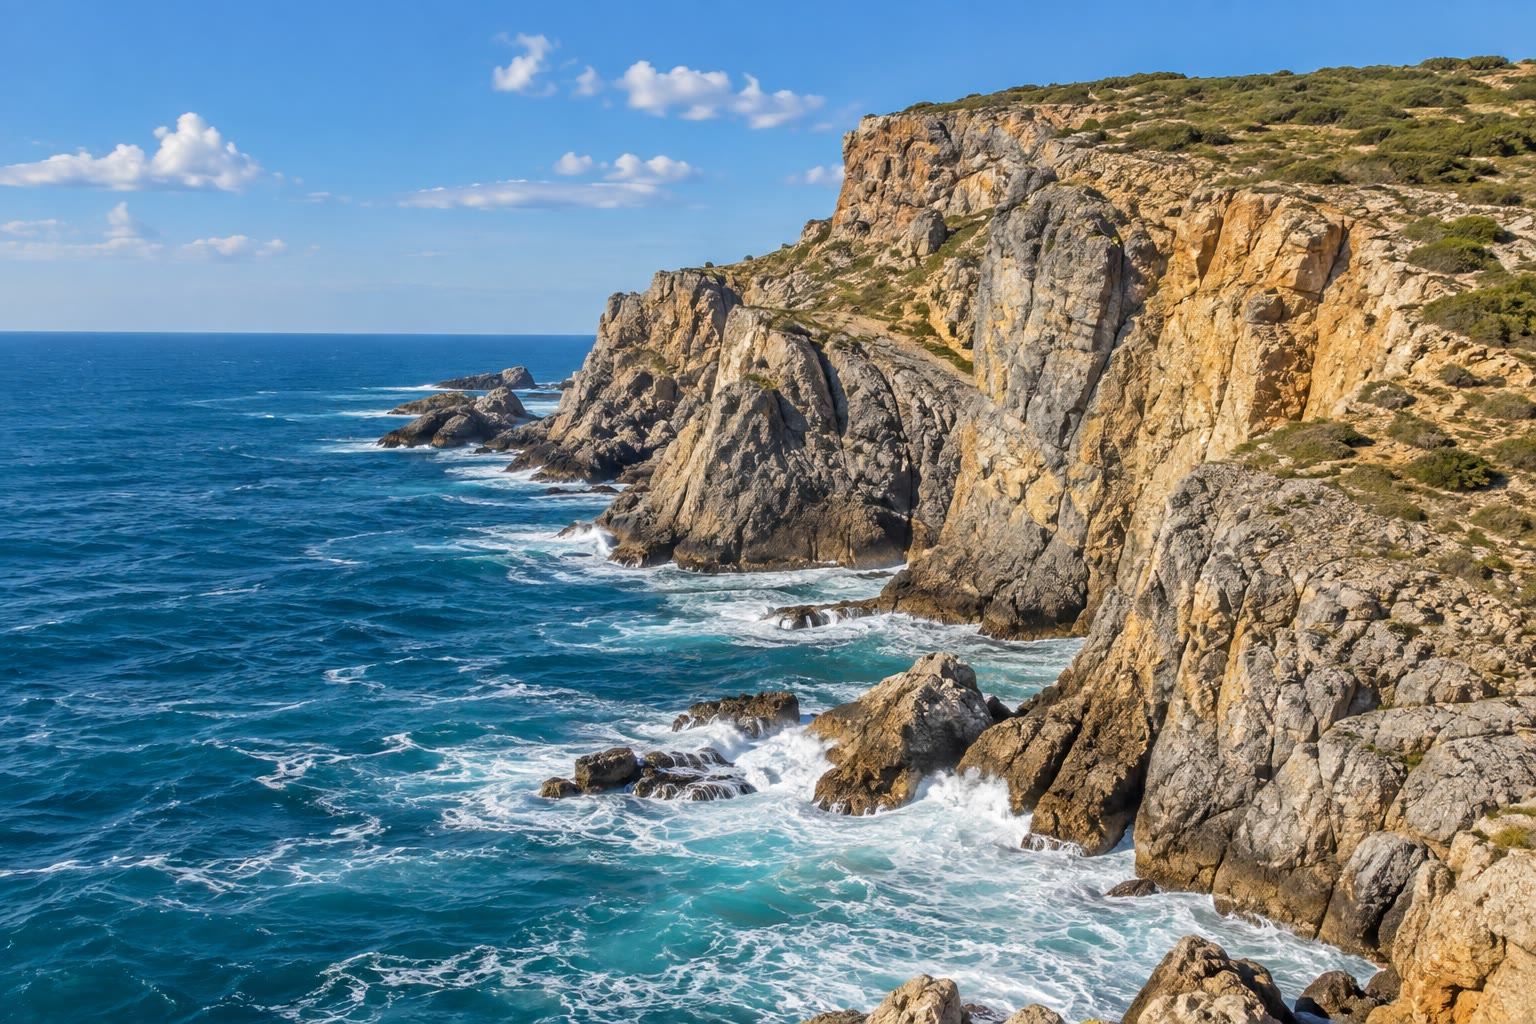
\includegraphics[width=0.55\linewidth]{images/book1/ai/g9-coastal-cliff.jpg}

{\small Roche, mer et \omterm{def:g4:air-a-mixture-of-gases:air}{air}~: trois \omterm{def:g6:pure-substances-and-mixtures:mixture}{mélanges} très différents des mêmes
éléments.}
\end{omfigure}

\section{Exercices}

\begin{exercise}[$\star$]\label{exo:g9:elements-universe-earth:1}
Quels sont les deux éléments qui forment presque tout le Soleil~?
\end{exercise}

\begin{exercise}[$\star$]\label{exo:g9:elements-universe-earth:2}
Quel est l'élément le plus abondant dans la croûte terrestre~? Dans le
corps humain (en masse)~?
\end{exercise}

\begin{exercise}[$\star$]\label{exo:g9:elements-universe-earth:3}
Où la plupart des éléments plus lourds que l'hélium ont-ils été
fabriqués~?
\end{exercise}

\begin{exercise}[$\star$]\label{exo:g9:elements-universe-earth:4}
Quel pourcentage de la masse de l'eau de mer est du sel dissous~?
\end{exercise}

\begin{exercise}[$\star\star$]\label{exo:g9:elements-universe-earth:5}
Sur le diagramme de la croûte, additionne les parts de l'oxygène et du
silicium. Quelle fraction de la croûte cela représente-t-il, à peu
près~?
\end{exercise}

\begin{exercise}[$\star\star$]\label{exo:g9:elements-universe-earth:6}
Pourquoi y a-t-il si peu d'hydrogène et d'hélium dans la croûte
terrestre, alors que le Soleil en est presque entièrement fait~?
\end{exercise}

\begin{exercise}[$\star\star$]\label{exo:g9:elements-universe-earth:7}
Quelle masse de carbone y a-t-il dans un corps de \qty{70}{kg} qui
contient \qty{23}{\percent} de carbone~?
\end{exercise}

\begin{exercise}[$\star\star$]\label{exo:g9:elements-universe-earth:8}
Pourquoi l'oxygène est-il l'élément le plus répandu dans le corps en
masse, alors que l'hydrogène est le plus répandu en nombre d'\omterm{def:g7:atoms-and-molecules:atom}{atomes}~?
\end{exercise}

\begin{exercise}[$\star\star$]\label{exo:g9:elements-universe-earth:9}
Un bloc de granite de \qty{1000}{kg} est un morceau typique de la
croûte. D'après le diagramme, quelle masse d'aluminium contient-il,
environ~?
\end{exercise}

\begin{exercise}[$\star\star$]\label{exo:g9:elements-universe-earth:10}
Quels éléments figurent parmi les principaux éléments à la fois de la
croûte et du corps humain~?
\end{exercise}

\begin{exercise}[$\star\star\star$]\label{exo:g9:elements-universe-earth:11}
Un corps de \qty{70}{kg} contient environ \qty{1.06}{kg} de calcium.
Calcule la masse d'un \omterm{def:g7:atoms-and-molecules:atom}{atome} de calcium ($A = 40$), puis le nombre
d'\omterm{def:g7:atoms-and-molecules:atom}{atomes} de calcium. Écris-le en écriture scientifique.
\end{exercise}

\begin{exercise}[$\star\star\star$]\label{exo:g9:elements-universe-earth:12}
Les \omterm{def:g7:atoms-and-molecules:atom}{atomes} de ton corps ont tous fait partie d'autres choses auparavant.
Utilise le voyage d'un \omterm{def:g7:atoms-and-molecules:atom}{atome} de carbone pour expliquer pourquoi le
nombre total d'\omterm{def:g7:atoms-and-molecules:atom}{atomes} de carbone sur la Terre ne change presque pas.
\end{exercise}

\section{Problème~: combien d'atomes suis-je~?}

\begin{problem}[{Problème du week-end --- d'un diagramme d'abondance au
nombre d'atomes d'oxygène d'un corps humain}]
\label{pb:g9:elements-universe-earth:1}
% ledger: body:atoms-O, body:atoms-total
Un adulte mince de \qty{70}{kg} contient, en masse, environ
\qty{61}{\percent} d'oxygène, \qty{23}{\percent} de carbone et
\qty{10}{\percent} d'hydrogène. On prendra pour masse d'un \omterm{def:g9:inside-the-atom:proton}{nucléon}
\qty{1.67e-27}{kg}~; un \omterm{def:g7:atoms-and-molecules:atom}{atome} d'oxygène compte 16 \omterm{def:g9:inside-the-atom:proton}{nucléons}, un \omterm{def:g7:atoms-and-molecules:atom}{atome} de
carbone 12, un \omterm{def:g7:atoms-and-molecules:atom}{atome} d'hydrogène 1. On néglige les \omterm{def:g9:inside-the-atom:nucleus}{électrons}.

\medskip
\noindent\textbf{Partie I --- Les masses.}
\begin{enumerate}
  \item Calcule la masse d'oxygène du corps.
  \item Calcule la masse de carbone et celle d'hydrogène.
  \item Quel pourcentage de la masse ces trois éléments représentent-ils
        ensemble~?
  \item La plus grande partie de cet oxygène et de cet hydrogène se
        trouve dans un même composé. Lequel~?
\end{enumerate}

\medskip
\noindent\textbf{Partie II --- Un seul \omterm{def:g7:atoms-and-molecules:atom}{atome}.}
\begin{enumerate}[resume]
  \item Calcule la masse d'un \omterm{def:g7:atoms-and-molecules:atom}{atome} d'oxygène.
  \item Calcule la masse d'un \omterm{def:g7:atoms-and-molecules:atom}{atome} de carbone et celle d'un \omterm{def:g7:atoms-and-molecules:atom}{atome}
        d'hydrogène.
  \item Combien d'\omterm{def:g7:atoms-and-molecules:atom}{atomes} d'hydrogène pèsent autant qu'un \omterm{def:g7:atoms-and-molecules:atom}{atome}
        d'oxygène~?
  \item Pourquoi peut-on négliger les \omterm{def:g9:inside-the-atom:nucleus}{électrons}~?
\end{enumerate}

\medskip
\noindent\textbf{Partie III --- Le décompte.}
\begin{enumerate}[resume]
  \item Calcule le nombre d'\omterm{def:g7:atoms-and-molecules:atom}{atomes} d'hydrogène du corps.
  \item Calcule le nombre d'\omterm{def:g7:atoms-and-molecules:atom}{atomes} de carbone.
  \item Calcule le nombre d'\omterm{def:g7:atoms-and-molecules:atom}{atomes} d'oxygène du corps.
  \item Une estimation soigneuse donne $1.61 \times 10^{27}$ \omterm{def:g7:atoms-and-molecules:atom}{atomes}
        d'oxygène dans un tel corps. Compare avec ton décompte, et donne
        le nombre d'\omterm{def:g7:atoms-and-molecules:atom}{atomes} d'oxygène d'un corps de \qty{70}{kg} avec deux
        chiffres significatifs.
\end{enumerate}
\end{problem}
